\documentclass[a4paper,english]{article}
\usepackage{babel}
\usepackage[utf8]{inputenc}
\usepackage[T1]{fontenc}
\usepackage{times}
\usepackage[pdftex]{graphicx}
\usepackage{color}
\usepackage[pdftex,colorlinks=true,citecolor=black,
            pagecolor=black,linkcolor=black,menucolor=black,
            urlcolor=black]{hyperref}
\usepackage{epstopdf} % addition to include eps
\usepackage{eufrak}
\usepackage{amsmath}
\usepackage{amsbsy}
\usepackage{eucal}
%\usepackage{caption}
%\usepackage{subcaption} % for subfigures
\usepackage{subfig}
\usepackage{longtable}
\usepackage{url}
\urlstyle{same}
\usepackage{setspace}
\usepackage{natbib}
\usepackage{listings}
\usepackage{algorithm, algorithmic}
\usepackage[version=3]{mhchem} % for chemical reactions

\pdfinfo{            
          /Title      (T-61.5110 Modeling of Biological Networks)
          /Author     (Arttu Modig)
          /Keywords   ()          
}


\title{T-61.5110 Modeling of Biological Networks \\ Exercise Session 7}
\author{Arttu Modig \\ 79358S \\
       {\it arttu.modig@aalto.fi}}


\begin{document}
%--- KANSILEHTI -------------------------------------------------------------
\maketitle


%\newpage
%------------------------------------------------------------------------------
\onehalfspacing
\section*{1. Deterministic to Stochastic model conversion}

The dynamics of two species are given as:
\[ \ce{2P1 -> P2} ,\]
\[ \ce{P2 -> 2P1} .\]

The Figure \ref{fig:dimer} shows a plot that models the deterministic interaction. We may see that the dynamics converge after Time > 8.

\begin{figure}[htp]
    \begin{center}
        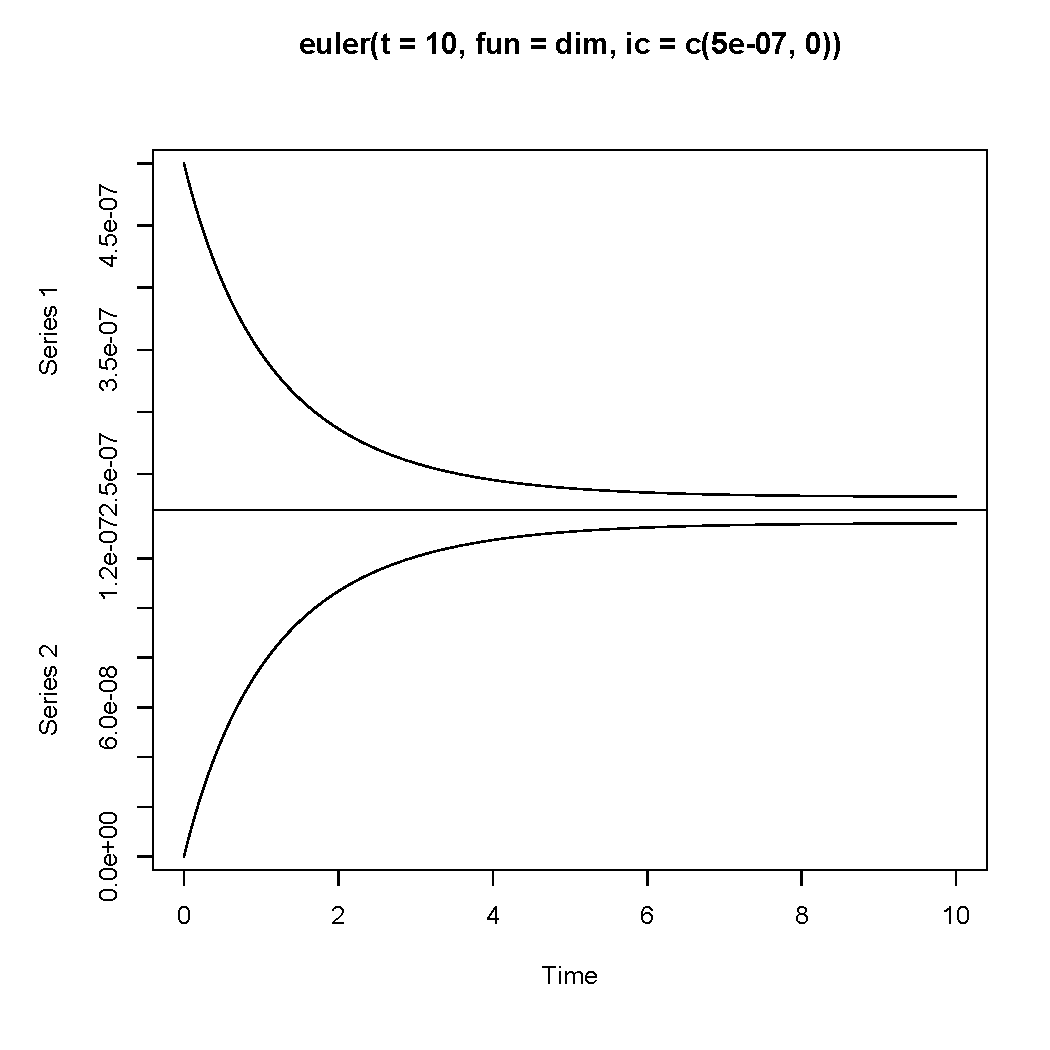
\includegraphics[width=0.5\textwidth]{dimer}
        \caption{The plot shows the deterministic dynamics of two species.}
        \label{fig:dimer}
    \end{center}
\end{figure}

\paragraph{b.}

The dynamics of the two species are now simulated using discrete stochastic kinetics. The repeated simulations are in Figure \ref{fig:stoch}. As we may see, there are some differences, and the dynamics won't converge because this is a probabilistic stochastic model.

\begin{figure}[htp]
  \centering
  \subfloat[Run 1]{\label{fig:1}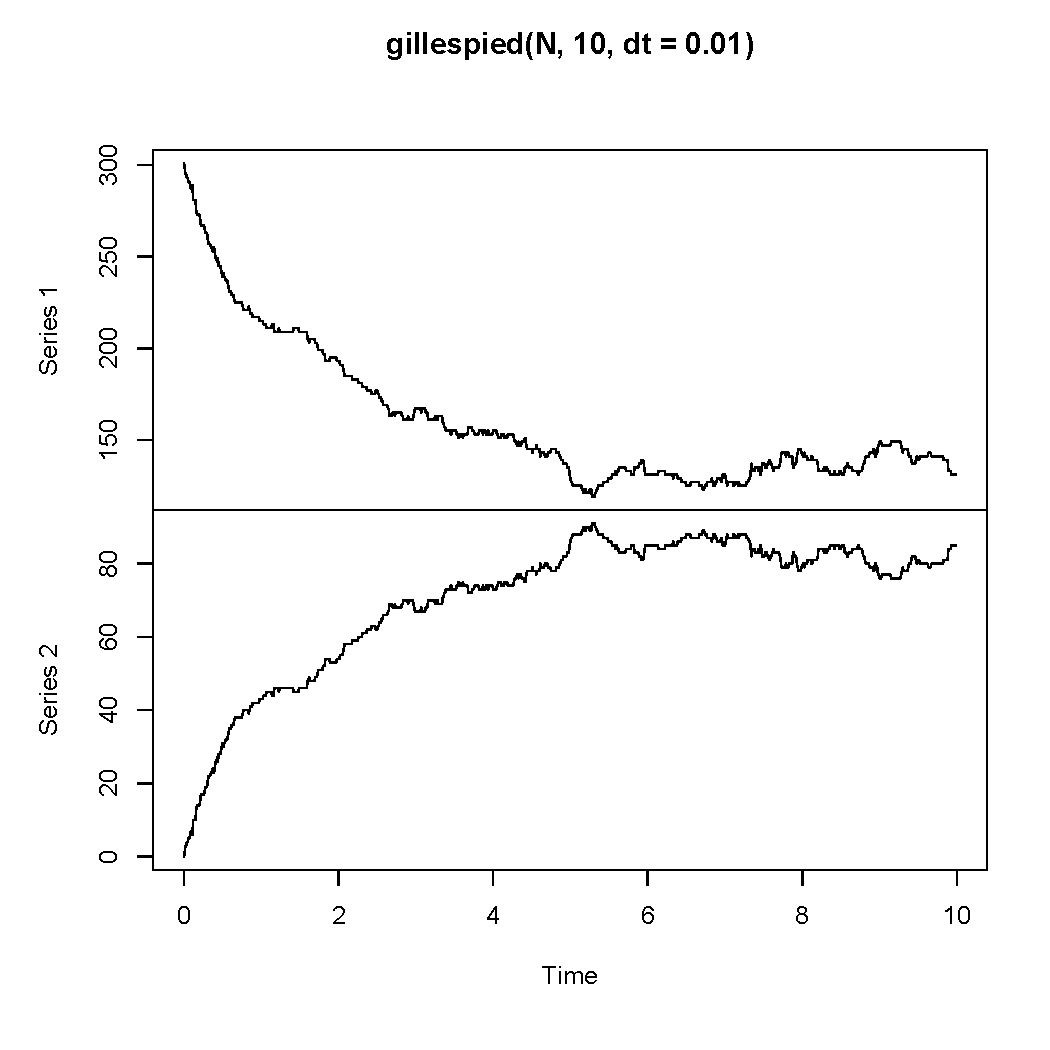
\includegraphics[width=0.4\textwidth]{dimer-stoch}}
  \subfloat[Run 2]{\label{fig:2}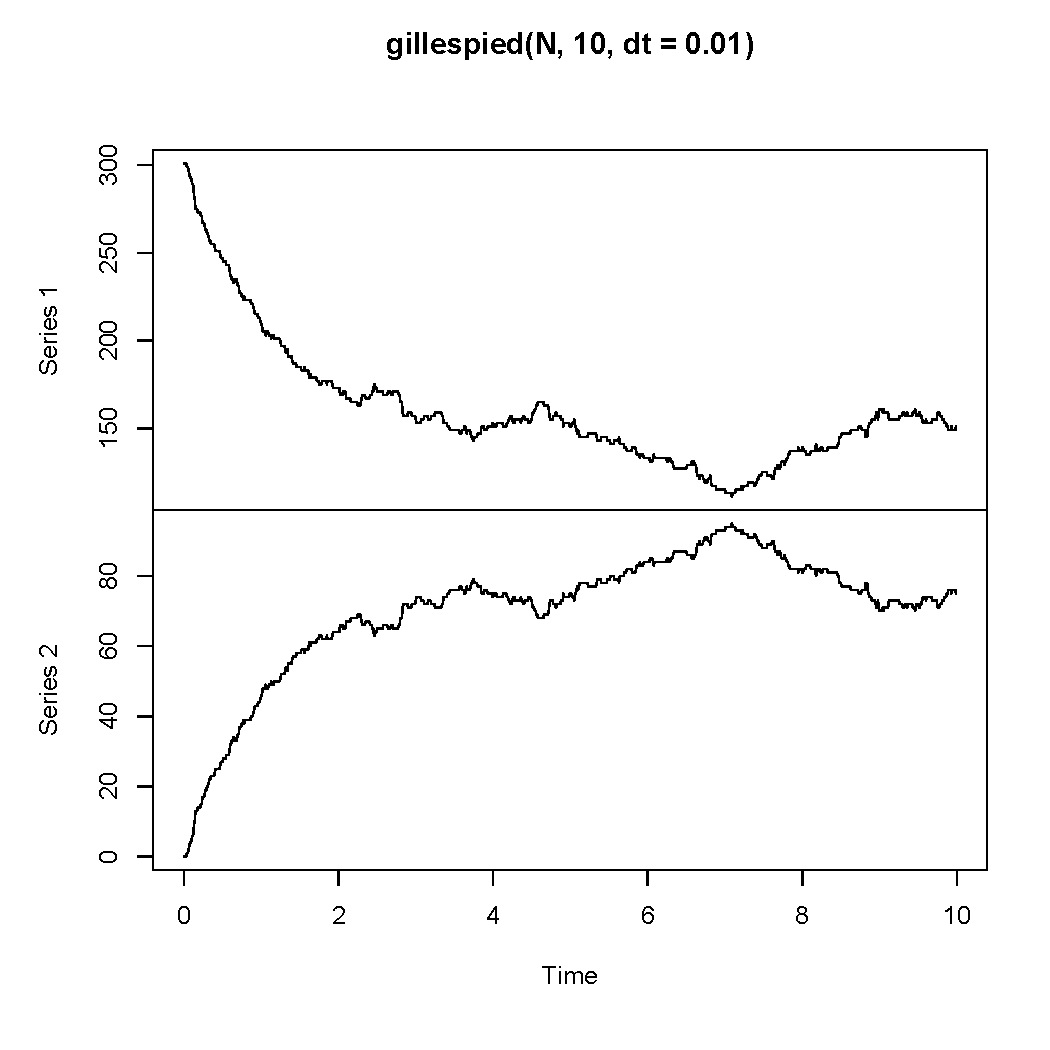
\includegraphics[width=0.4\textwidth]{dimer-stoch2}}
  \\
  \subfloat[Run 3]{\label{fig:3}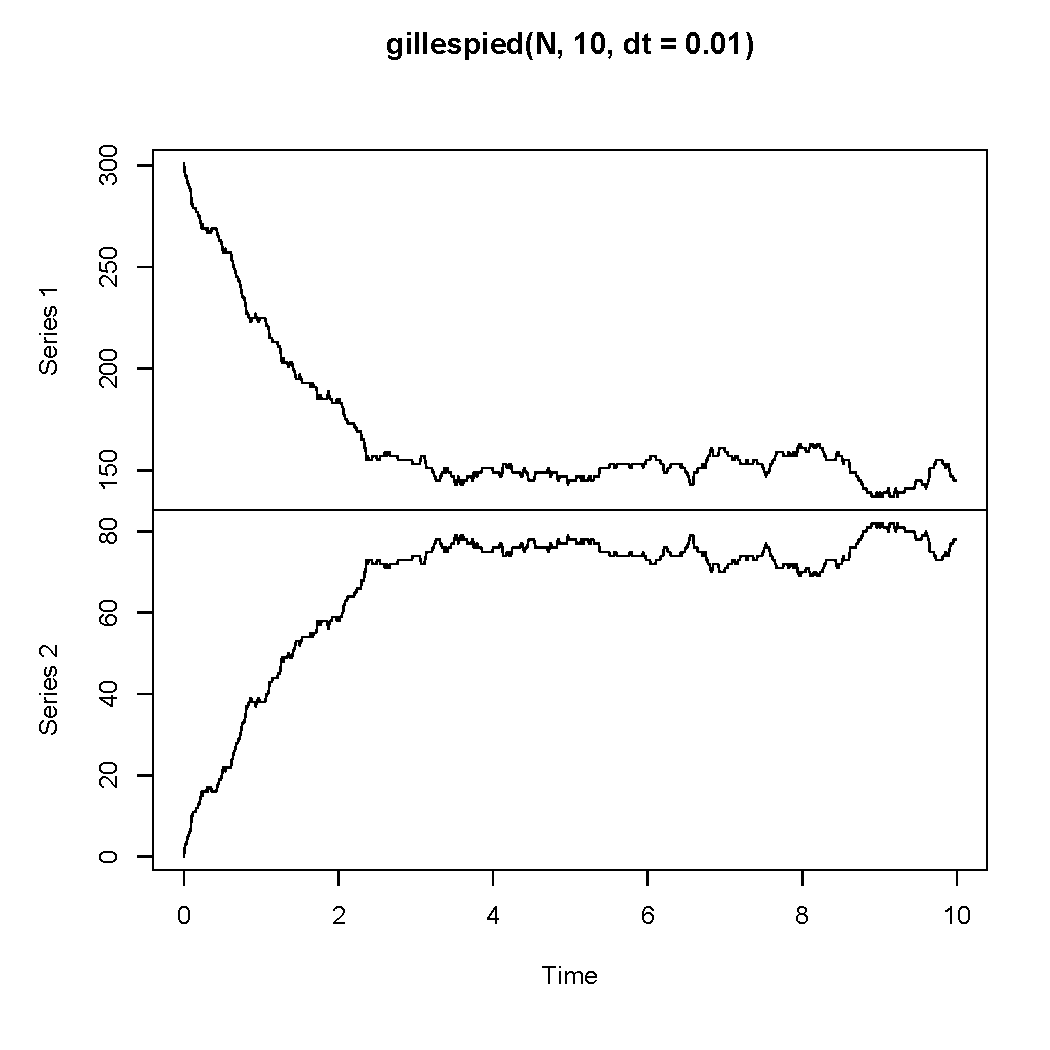
\includegraphics[width=0.4\textwidth]{dimer-stoch3}}
  \subfloat[Run 3]{\label{fig:3}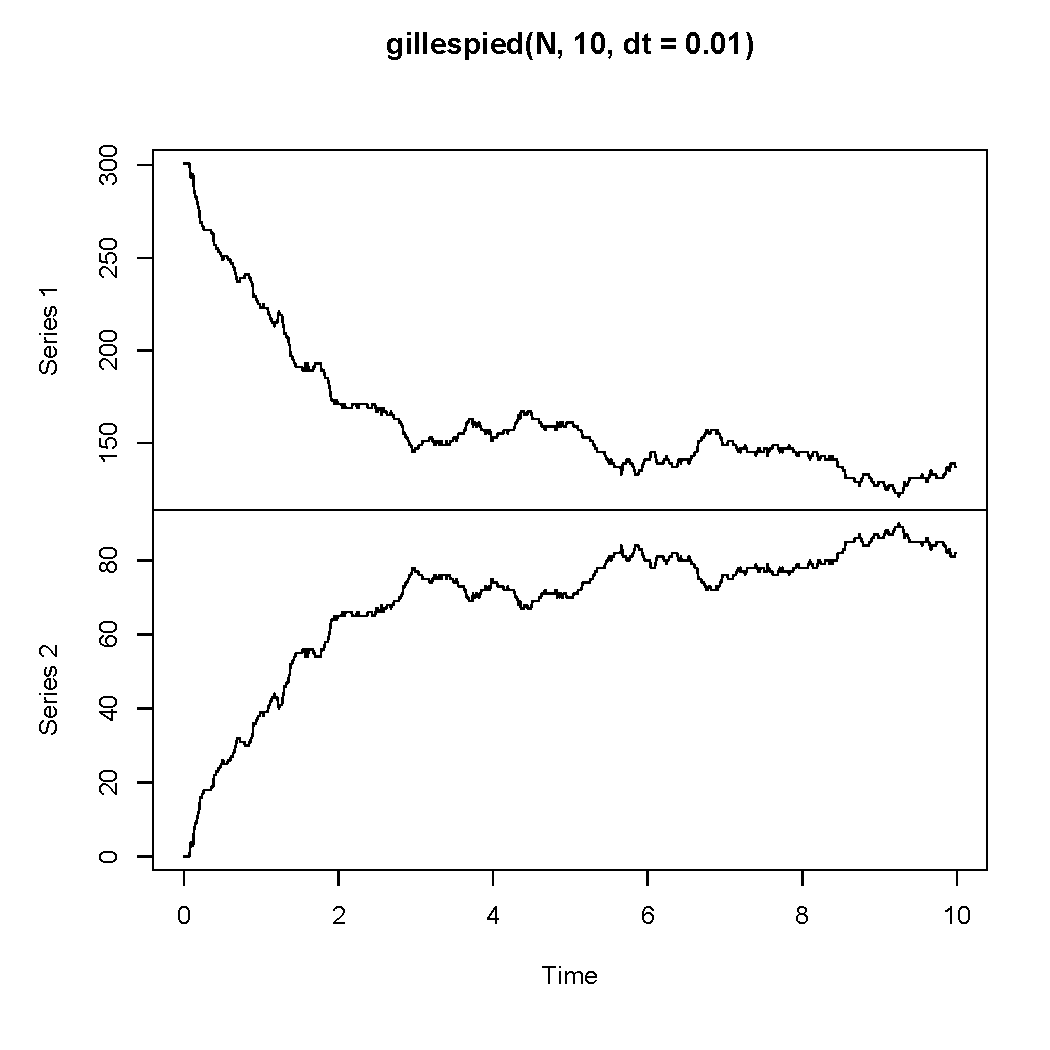
\includegraphics[width=0.4\textwidth]{dimer-stoch4}}
  \caption{The plots show several runs of the stochastic dynamics of two species.}\label{fig:stoch}

\end{figure}

\paragraph{c.}

We now run the stochastic simulator 1000 times, and compare the number of molecules. The simulation plots are drawn on Figure 3\subref{fig:sim1}, and the sample mean with confidence intervals are on Figure 3\subref{fig:sim2}. A histogram of the amount of molecules on time T=20 is shown on Figure 3\subref{fig:sim3}.


\begin{figure}[htp]
  \centering

  \subfloat[Number of molecules with 1000 simulations.]{\label{fig:sim1}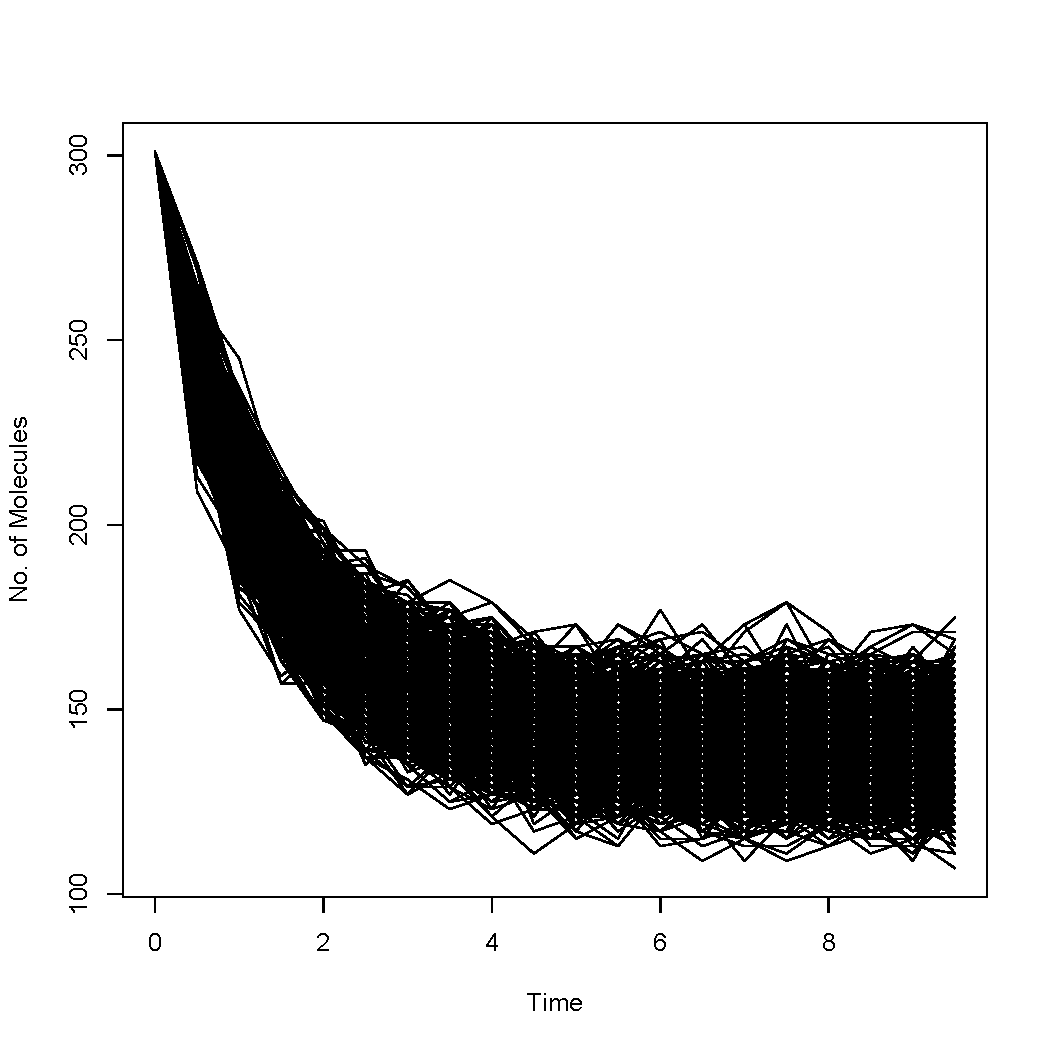
\includegraphics[width=0.4\textwidth]{samples}}
  \subfloat[The mean of number of molecules with 1000 simulations.]{\label{fig:sim2}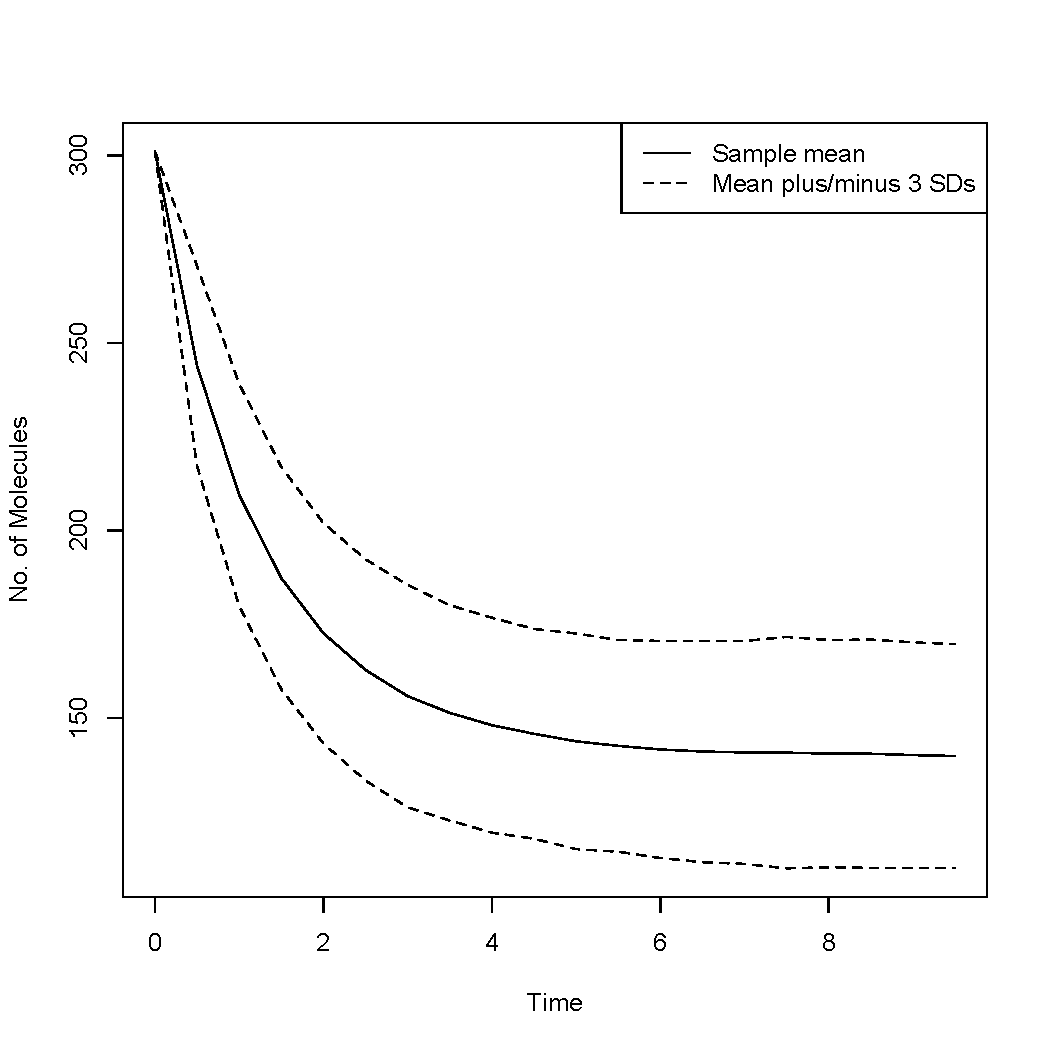
\includegraphics[width=0.4\textwidth]{samplemean}}
  \\
  \subfloat[Number of molecules at time T=20.]{\label{fig:sim3}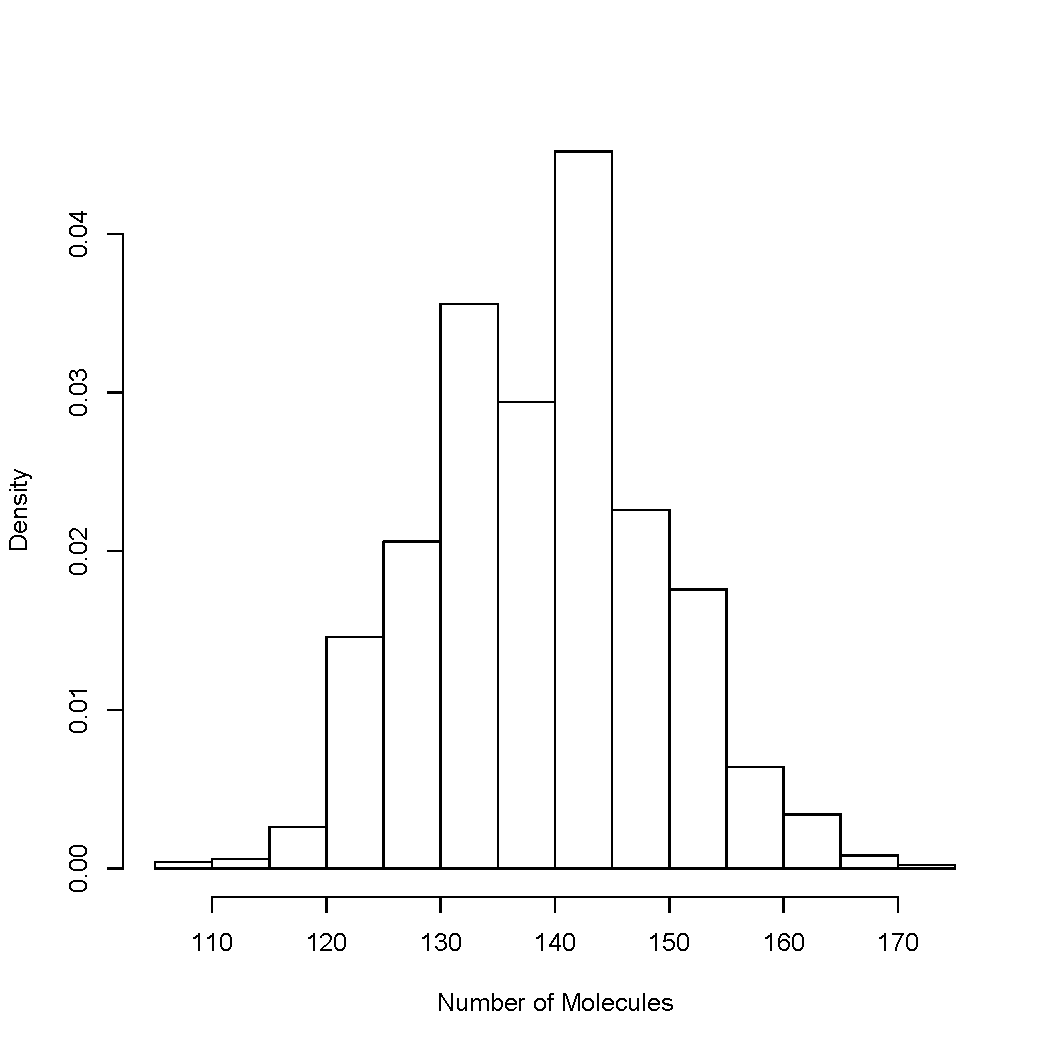
\includegraphics[width=0.4\textwidth]{hist}}
  \caption{The plots for the Assignment 1(c).}\label{fig:sim}
  
\end{figure}

\section*{2. Stochastic models: Uncertainty and Sensitivity analysis}

The stochastic simulator is run again, but now we have uncertainty about about value $k_2$. The new results are shown on Figure \ref{fig:sim-2}. We can see that the distribution mean is moved further, to about 150 molecules at time T=20, when in the case $k_2$ the mean was under the 150.

\begin{figure}[htp]
  \centering

  \subfloat[Number of molecules with 1000 simulations.]{\label{fig:sim-2-1}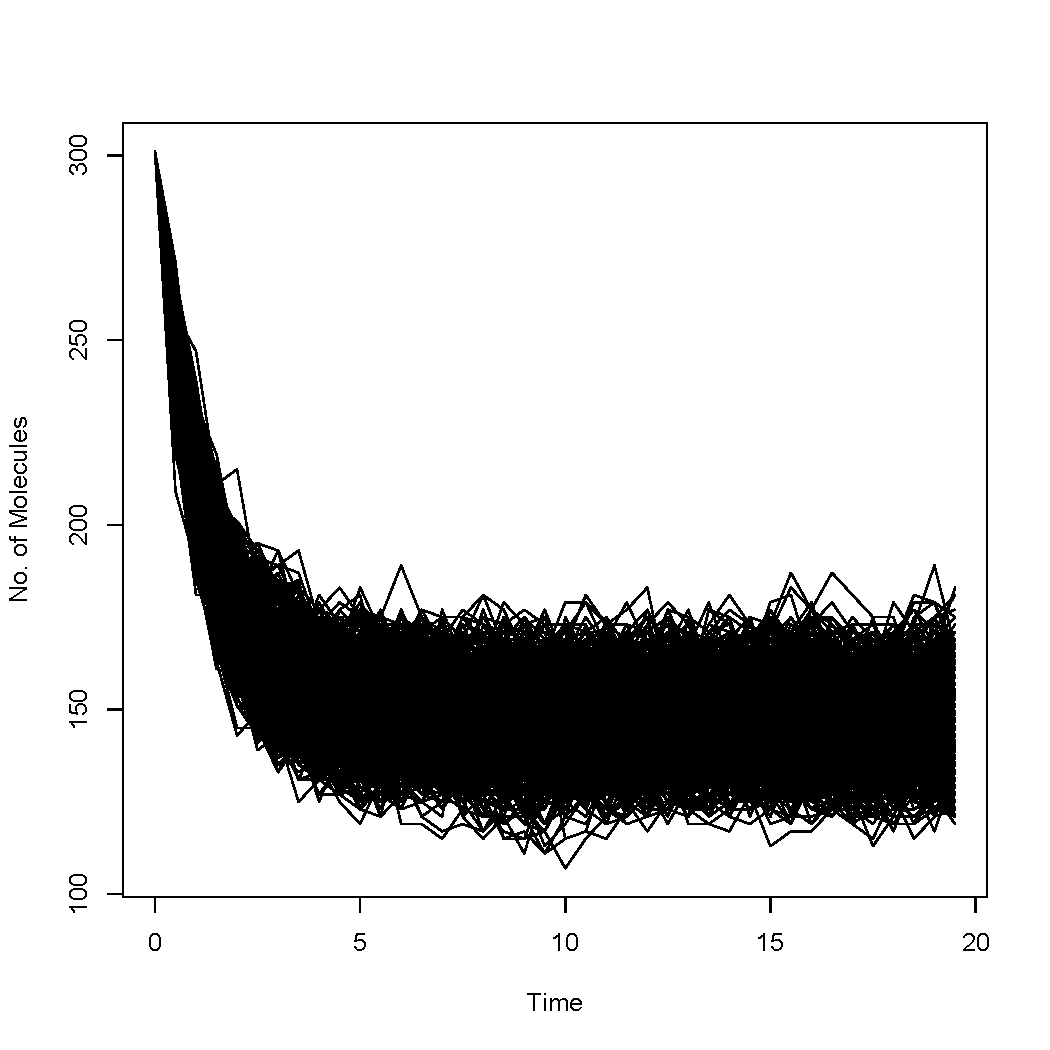
\includegraphics[width=0.4\textwidth]{samples2}}
  \subfloat[The mean of number of molecules with 1000 simulations.]{\label{fig:sim-2-2}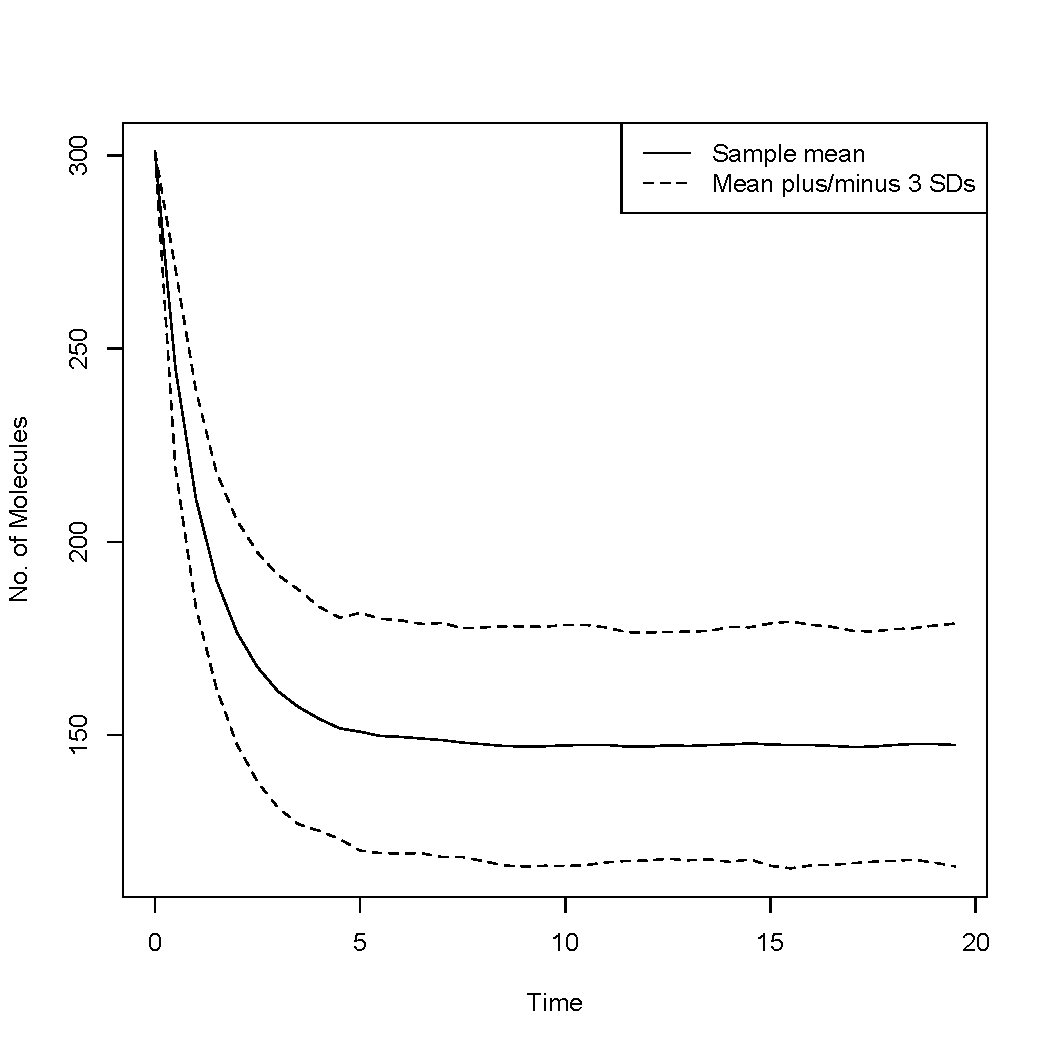
\includegraphics[width=0.4\textwidth]{samplemean2}}
  \\
  \subfloat[Number of molecules at time T=20.]{\label{fig:sim-2-3}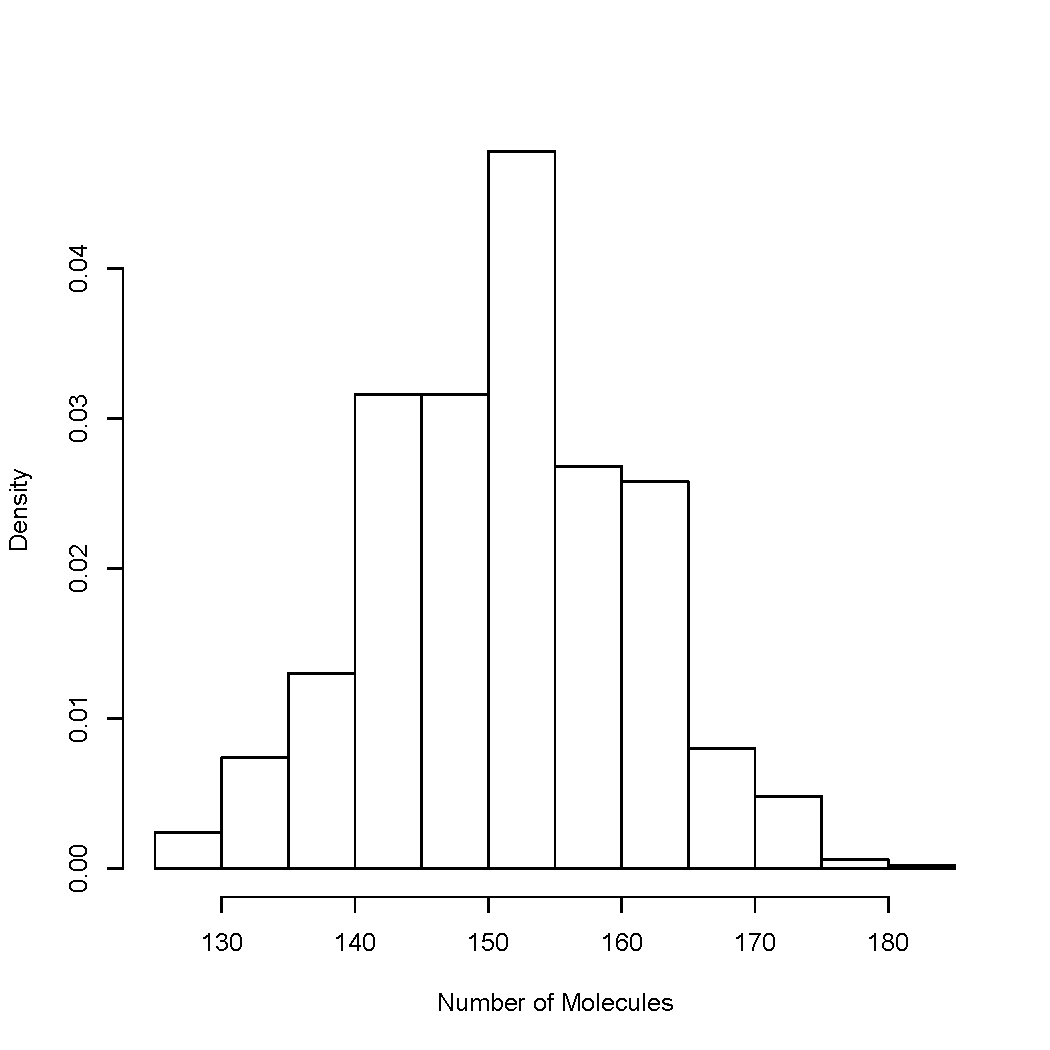
\includegraphics[width=0.4\textwidth]{hist2}}
  \caption{The plots for the Assignment 2.}\label{fig:sim-2}
  
\end{figure}


\end{document}

%%% Local Variables: 
%%% mode: latex
%%% TeX-master: t
%%% End: 
